\chapter{Introduction}
\label{introchap}

\section{Motivation}
\sectionmark{Motivation}

\subsection{Convection in astrophysics: Stars \& Beyond}
\label{sct:convective_abundance}
In nature, thermal buoyancy forces primarily drive two types of flows: gravity waves and convection.
Gravity waves are driven when the atmospheric or fluid stratification is convectively \emph{stable}.
Convection is the opposite, and is the manifestation of these buoyancy forces in the presence of an \emph{unstable} or \emph{superadiabatic} stratification.
Convection occurs in the Earth's atmosphere, and cumulus clouds are evidence of that convection (and there is a rich literature investigating atmospheric convection, see \citet{yano2014} for a recent review).
The Earth's mantle convects \citep{schubert&all2001}, driving plate tectonics \citep{bercovici2003}, and the earth's outer core convects, driving the Earth's magnetic dynamo \citep{christensen2011}.
Convection also accurs in more exotic astrophysical systems, including in the planes of accretion disks \citep{held&latter2018} and in the magnetospheres of giant planets \citep{thomsen&all2012}.
The prevelance of convective motions across astrophysics suggests that an intricate understanding of the fundamental nature of convection is crucial.

One of the most classical and well-studied examples of astrophysical convection is convection in stars.
The surface of the Sun is covered in convective ``granules,'' and these granules are evidence of a convection zone that occupies the outer 30\% of the Sun's radial profile \citep{miesch2005, nordlund&all2009}.
The Sun is not the only Main Sequence (MS) star to rely on convection to transport a part of its luminosity.
``Early-type'' or ``Upper-MS'' high-mass stars ($M \gtrsim 1.5 M_\odot$, where $M_\odot$ is the solar mass) have convecting regions in their cores.
In these massive stars, core conditions are sufficiently extreme that the CNO cycle is activated.
The opacity of the stellar material, dominated by free-free interactions \citep[c.f.~Ch.~16 of][]{weiss&all2004}, is sufficiently high that the extreme CNO-fed luminosities cannot be efficiently carried by radiative processes.
Convection is therefore required to transport the stellar luminosity outward, and results in a well-mixed convective core region.
The luminosity of stars with masses smaller than $1.5 M_\odot$ is provided by the pp-chain, and these stars have stable cores.
However, these stars also have cooler surface temperatures which allow for phase changes of hydrogen and helium within their stellar envelopes.
These elements are the primary consitutents of the stellar material, and unionized atoms greatly increase the stellar opacity through bound-free (photo effect) interactions \citep[these effects were first studied in detail by ][]{rast&toomre1993a, rast&toomre1993b}.
In solar-type stars ($1.5 M_\odot \lesssim M \lesssim 0.3 M_\odot$), this increased opacity near the stellar surface results in a convectively unstable envelope which overlies a stable, radiative interior.
In ``Late-type'', ``Lower-MS'' stars, these opacity effects lead to convective instability throughout the full depth of the star.
While stars spend the majority of their lifetimes on the MS, convection is also an important process during other evolutionary phases \citep[and I refer the reader to chapter 2 of][for a broad but brief overview of stellar evolutionary phases]{HKT}.

The relatively new fields of helioseismology and asteroseismology (briefly explored in Sct.~\ref{sct:asteroseismology}) have enabled scientists to literally look inside of the Sun and stars.
These measurements allow us to put constraints upon and test the validity of stellar structure models, and our assumptions about the workings of stellar interiors.
In Sct.~\ref{sct:convective_conundrum}, I briefly discuss the ``Solar Convective Conundrum,'' one of the discrepancies between models and observations that has been revealed by helioseismology.
In short, this conundrum shows that our fundamental understanding of stellar convection is flawed.
The collection of experiments presented in this thesis were largely motivated by this Conundrum, and a desire to rebuild some understanding of stellar convection from fundamental principles.

\subsection{Asteroseismology \& Helioseismology}
\label{sct:asteroseismology}
Stars are seismically active.
This seismic activity is the manifestation of complex, 3D oscillations within the star which come in two primary forms: pressure-driven ``p''-modes, and buoyancy-driven ``g''-modes.
The simplest of these modes are radial modes, in which the star experiences spherically symmetric oscillations along its radial coordinate (and the simplest of these modes is the fundamental ``breathing'' mode, in which the star's radius expands and contracts as a whole).
On top of these radial modes, nonradial modes (including dipolar, quadrupolar, and infinitely more complex modes) are also excited.
As these nonradial modes propagate into the stellar interior, the stratification of the star (e.g., the changing sound speed with depth for the p-modes) causes the waves to refract and return to the surface.
These waves therefore directly sample the interior stratification of the star, and modes with higher spherical harmonic degrees probe different depths.
Asteroseismology and helioseismology refer to the observation of wavefields at the surface of stars, or the Sun, respectively.
Asteroseismology can only detect a limited number of modes due to the fact that stars are not spatially resolved.
On the other hand, helioseismology, which probes the interior of the Sun, has access to high-resolution spatial data and can theoretically detect a large range of modes.
Helioseismic and asteroseismic theory, observations, and applications have respectively been covered extensively by \cite{christensen-dalsgaard2002} and \cite{aerts&all2010}.

The advent of asteroseismic science has closely paralleled that of exoplanetary science.
Early ground-based observations of stellar pulsations \cite[e.g.,][]{kjeldsen&frandsen1991, bouchy&carrier2001, bedding&all2001} have given way to datasets larger than $10^4$ stars \cite[e.g.,][]{yu&all2018, santos&all2019b} in the age of CoRoT, Kepler, and K2 data.
Another 20,000 asteroseismically-interesting targets are being observed in the TESS satellite's two-year mission \citep{schofield&all2019}.
By 2030 we expect to have observed $10^7$ pulsating red giants and $10^5$ dwarfs and subgiants \citep{huber&all2019}.
In addition to teaching us about the nature of stellar interiors, asteroseismology enables the accurate measurement of stellar ages, masses, and radii, which in turn facilitates studies in galactic archaeology and exoplanetary measurements.

Going from asteroseismic data to a stellar structure model is difficult due to the small number of measurable frequencies available.
Forward modeling using one-dimensional (1D) stellar structure models is also difficult due to the need to recompute a stellar structure for each mass and age of star.
For a more complete discussion of the difficulties of inverse problems, we refer the reader to chs.~1.4 \& 4.1 of \citet{bellingerT2018}.
[TODO: Be more specific] As a general rule, 1D stellar structure models frequently fail to line up perfectly with asteroseismic measurements.
Some of the known deficiences of stellar structure models are described by \cite{buldgen2019}, and of particular interest in the context of this thesis are their handling of three-dimensional (3D) dynamical phenomena like convection.
The exponential rise in asteroseismic targets demands improved stellar structure models for comparison with asteroseismic datasets.
In order to improve these models, we must improve the handling of convection in stelar structure models. 

\begin{figure}[ht]
\includegraphics[width=\textwidth]{./figs/intro/asteroseismology.pdf}
\caption[Solar velocity power spectra.]
{
	Select images describing asteroseismology, taken from Ch.~1 of \citet{aerts&all2010}.
	(left, Fig.~1.6) Allowed frequency modes in a standard solar model.
	The upper part of the diagram is filled with p modes; frequency increases with overtone $n$ and spherical harmonic degree $\ell$.
	The lower part of the diagram is filled with g modes, whose frequency decreases with overtone $n$.
	(middle, Fig.~1.7a) Propagation of rays of sound waves in a cross-section of a Sun-like star.
	Shown are rays (in increasing order of penetration depth) of spherical harmonic degree of $\ell = \{75, 25, 20, 2\}$.
	(right, Fig.~1.9) A power spectrum of radial velocity variations for 9.5 years of data of the Sun-seen-as-a-star.
	Distinct peaks corresponding to p-modes (as in the left panel) can be seen.
	\label{fig:asteroseismology} 
}
\end{figure}



\subsection{The Solar Convective Conundrum}
\label{sct:convective_conundrum}
The outer 30\% of the Sun is a highly stratified convective envelope, and recent observations reveal that we lack a fundamental understanding of dynamics in this region.
Various helioseismic observations \citep{hanasoge&all2012, greer&all2015} detect convective velocity magnitudes which vary by two orders of magnitude.
Furthermore, these observations, as well as measurements of solar surface velocities \citep{hathaway&all2015}, have an unexpected absence of velocity at large spatial scales.
In short, we do not observe large-scale ``giant cells'' driven by buoyant motions deep in the solar convection zone.
These measurements, and the absence of giant cells, consitute the Solar Convective Conundrum.

Two primary hypotheses currently aim to explain the absence of giant cells: ``entropy rain'' and a rotationally constrained solar convective interior.
The entropy rain hypothesis, first suggested by \cite{spruit1997}, posits many theories over-predict the importance of upflows and that \emph{downflows} are predominantly responsible for carrying the solar luminosity across the solar convection zone.
Recent theory and simulations, including some of my own work, suggest that small, intense downflows can indeed traverse the entire convection zone intact and may be more important than upflows in solar-like convection \citep{brandenburg2016, kapyla&all2017, andersLB2019}.
To date, this work neglects magnetism and rotation, and it is unclear how these complicating effects interact with these fast, powerful downflows.
Meanwhile, the rotationally constrained interior hypothesis suggests that Coriolis forces dominate the dynamics of deep solar convection, and that these forces mask giant cells.
Simulations by \cite{featherstone&hindman2016} show that as convective flows become more rotationally constrained, dominant convective velocities are pushed to smaller length scales.
However, rotational effects on simulations can be hard to quantify; some simulations which nominally rotate at the solar rate show \emph{anti-solar} differential rotation \citep{gastine&all2014}, and other rotationally constrained simulations exhibit Jupiter-like bands \citep{brun&all2017}.
Regardless, current results and hypotheses suggest that the interplay between downflows and rotational effects must be better understood in stellar convection.

\begin{figure}[ht]
\includegraphics[width=\textwidth]{./figs/intro/conv_conundrum.pdf}
\caption[Solar velocity power spectra.]
{
	\citep[a, annoted Fig.~3 from][]{greer&all2015} Ring-diagram helioseismic observations of the solar velocity power spectrum at various depths.
	Here, velocity power decreases toward larger scales, unlike what is expected from simulations.
	\citep[b, annotated Fig.~8 from][]{hathaway&all2015} A spectrum of horizontal velocities at the solar surface, obtained using line-of-sight Doppler velocities.
	The length scales of surface granules and deeper supergranules appear as distinct features, but the hypothesized giant cells are not observed at low wavenumber.
	\label{fig:conv_conundrum} 
}
\end{figure}

\begin{figure}[ht!]
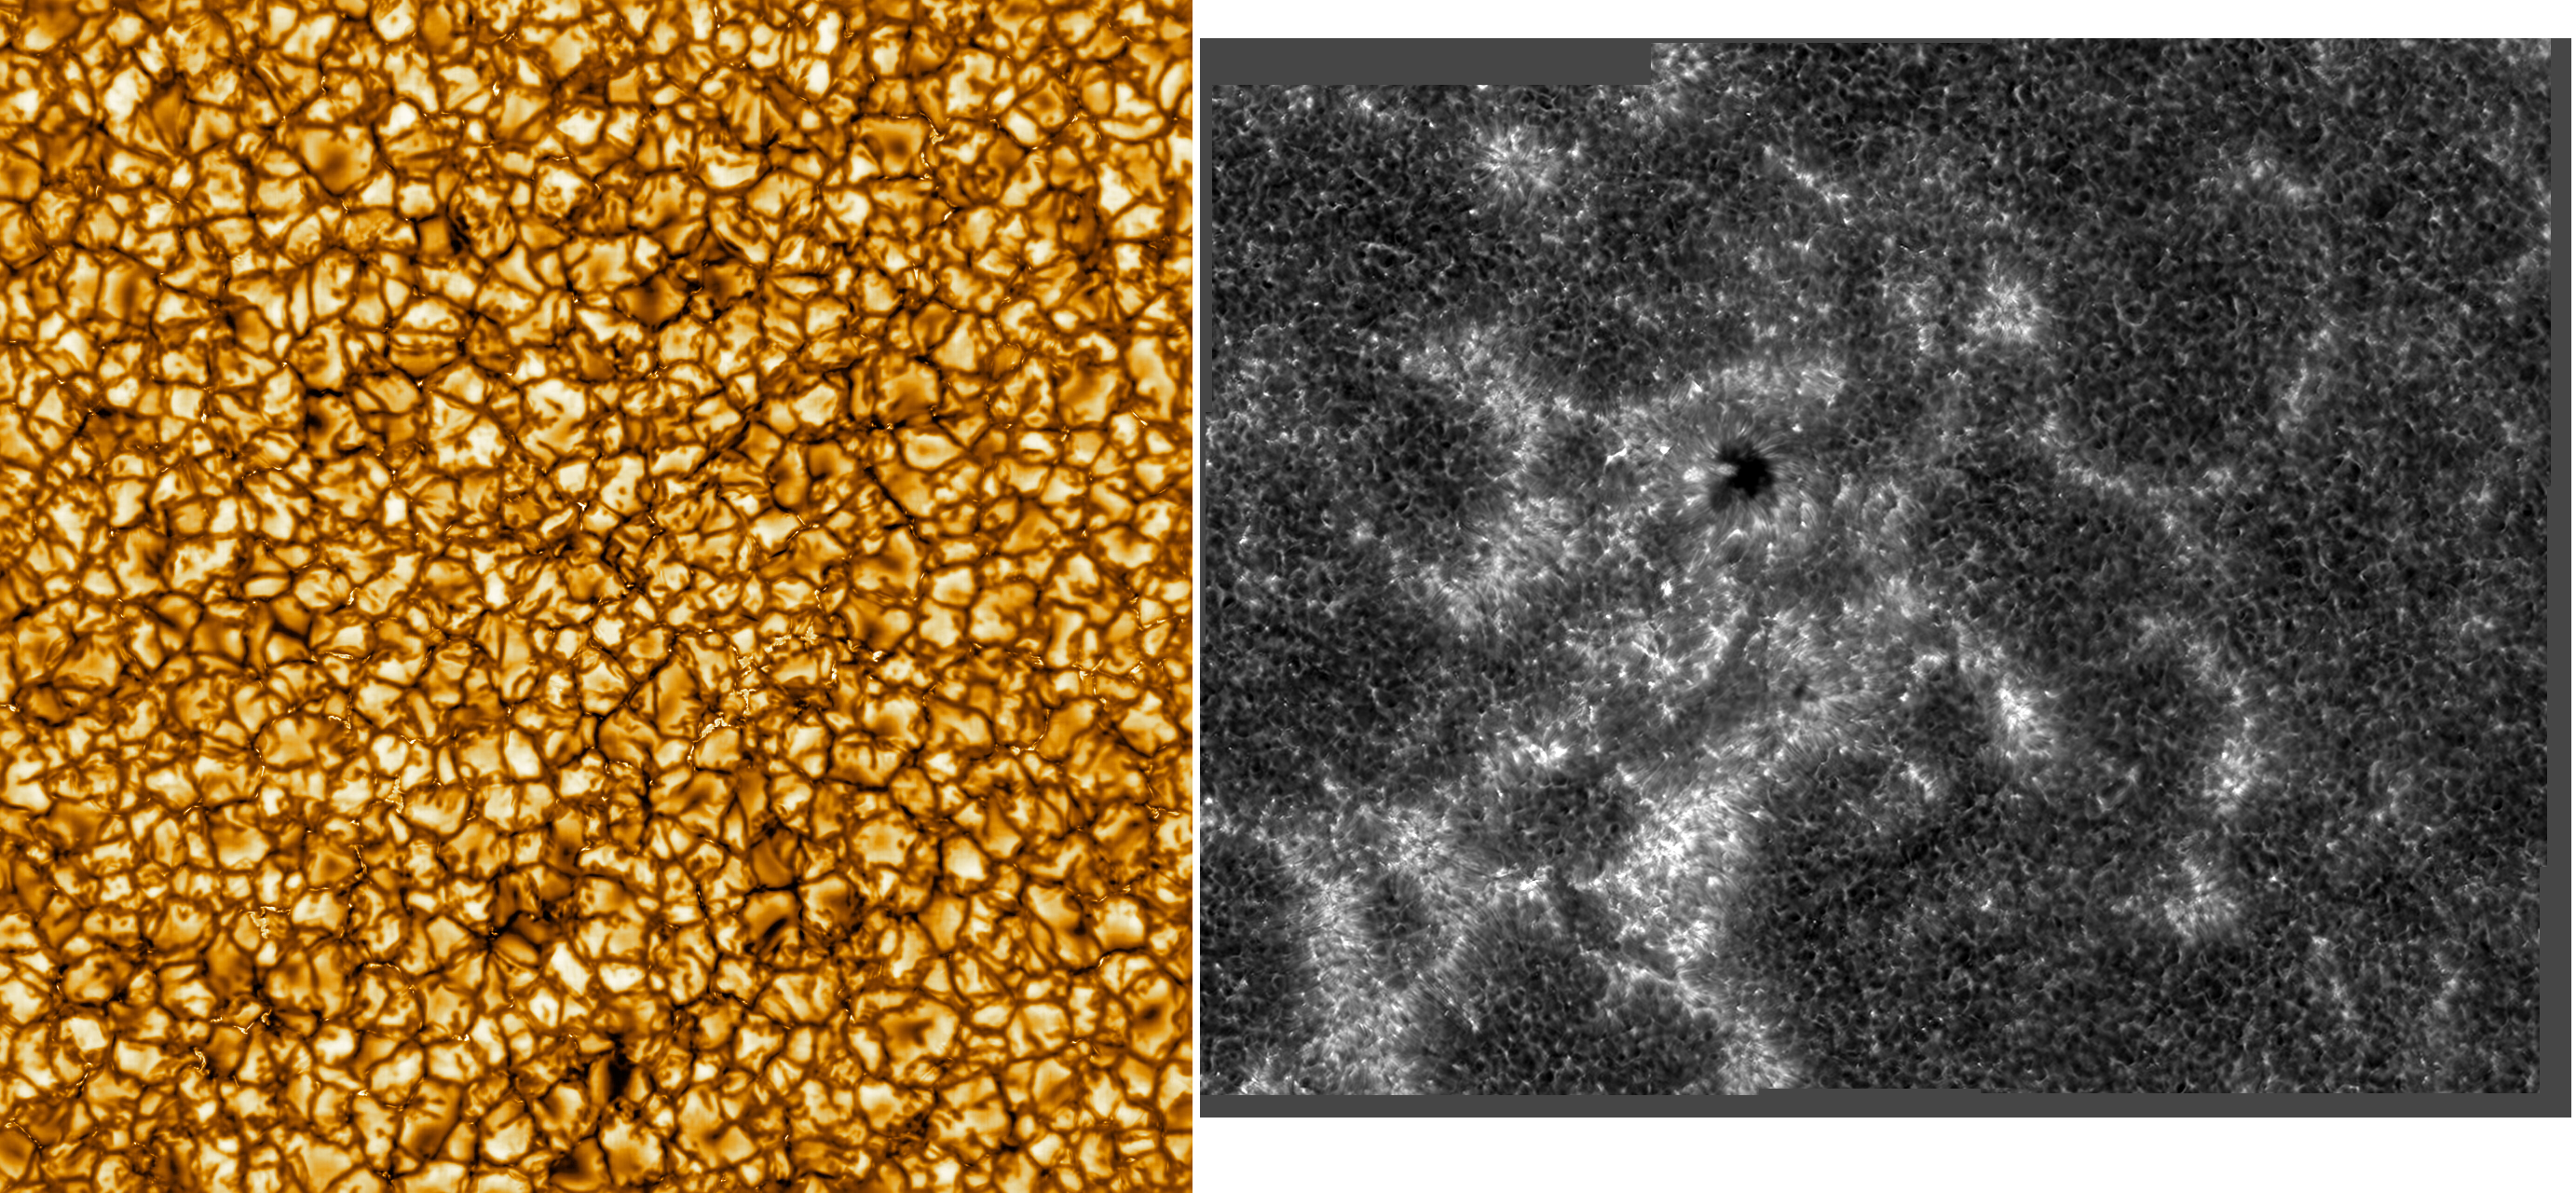
\includegraphics[width=\textwidth]{./figs/intro/solar_convection_scales.pdf}
\caption[Solar velocity power spectra.]
{
	(left) first-light image of the solar surface from DKIST (visible light [789 nm], covering 36.5 km$^2$).
	Bright, hot granules and relatively cool, dark intergranular lanes can be observed.
	Bright points occupying the center of intergranular lanes can also be seen \citep{vankooten&cranmer2017}.
	(right) Image of the solar surface from the Dutch Open Telescope (Ca II H line [396.8 nm]).
	The small-scale ``web'' of lights in this image trace out intergranular lanes.
	The large-scale web of lights roughly traces out the outlines of supergranules, the largest scale of convection that is observed at the solar surface.
	\label{fig:solar_convection_scales} 
}
\end{figure}




\section{A historical perspective on studies of convection}



\subsection{Laboratory Experiments \& Numerical Simulations}
The first controlled laboratory experiments of convection were performed by B\'{e}nard in 1900.


The earliest simulations in stellar-like convection \citep{graham1975, hurlburt&all1984, cattaneo&all1991, brummell&all1996, brummell&all1998} often sought to study simplified systems.
Cartesian geometry was employed, and convective flows in the presence of one or more complicating effects (stratification, rotation, magnetism, etc.)~were explored.
Despite vast modern computational resources, similar studies \cite[e.g.,][]{wood&brummell2012, anders&brown2017, wood&brummell2018} have become rare in the past two decades, and the highly laminar results of simulations from twenty years ago are often the state-of-the-art.

Recently, numericists have often switched aims from simply understanding convection to trying to reproduce precisely aspects of solar or stellar convection.
Small scale ``local'' simulations with realistic radiative transfer strikingly visually resemble solar surface convection and sunspots \citep{stein&nordlund1998, rempel&all2009, stein&nordlund2012, rempel2014}.
Local simulations have shaped how some observational experts interact with simulations, and the raw data of \cite{rempel2014}'s simulations are being used directly as high-resolution observations of solar convection \cite[see e.g.,][and others]{vankooten&cranmer2017, shchukina&trujillo2019}.
While simulations of solar surface convection reproduce solar features remarkably well, simulations of deep convection fail to reproduce observations  \citep{hanasoge&all2015}.
These global simulations exhibit giant cells as well as cycling dynamos and latitudinal differential rotation with very different timescales and profiles than those of the Sun \citep{brown&all2010, brown&all2011, guerrero&all2016, hotta&all2016, brun&all2017, strugarek&all2018}.
Simple simulations, where effects like rotation and magnetism can be well understood, should be utilized to understand why deep global simulations fail to reproduce solar observations.
This understanding can in turn be used to produce better ``realistic'' simulations which more accurately reflect aspects of true solar convection.
Realistic simulations built on a more detailed fundamental understanding of stellar convection can produce valuable synthetic observables for helioseismologists, asteroseismologists, and scientists who will soon use the NSF's Daniel K. Inouye Solar Telescope (DKIST) to study the solar surface at high resolution.


\subsection{Mixing Length Theory \& Stellar Structure Models}
The first analytical description of convection was performed by \citet{rayleigh1916}.
The earliest rudimentary Mixing Length Theory was derived by \citet{prandtl1925}.
One of the earliest formulations of a stellar mixing length theory was formulated by \citet{bohm-vitense1958}.
Modern MLT has many branches, but the one described in Chapter 14 of \citet{weiss&all2004} and early versions of that book are a fundamental description.

State-of-the-art stellar strucuture models are produced by 1D codes like MESA \citep{paxton&all2011}.
Unfortunately, MESA models necessarily depend on 1D parameterizations of convection and often employ the decades-old mixing length theory \cite[MLT,][]{bohm-vitense1958}.
While some aspects of convection are adequately described by MLT, it fails in a number of situations.
For example, 1D stellar models incorrectly produce pulsations in the surface layers of Sun-like stars, while 3D models of convection in these layers fare better \citep{jorgensen&weiss2019}.
Additionally, 1D models assume spherical symmetry and generally neglect magnetic and rotational effects.
Observations of stellar flares \citep{kowalski2016} and magnetically-induced pulsational frequency shifts \citep{santos&all2018} suggest that magnetism should not be neglected.
Furthermore, the Sun exhibits differential rotation characterized by latitudinal variations in angular velocity within the solar convection zone \citep{thompson&all1996, schou&all1998}, and latitudinal differential rotation has now been observed in other stars \citep{benomar&all2018}.
Together, these observations suggest that 1D parameterizations of convection which neglect complicating effects cannot sufficiently capture the complexities of stars.
In order to properly and fully utilize abundant asteroseismic data, we must improve the models on which asteroseismic inversions rely.


\section{Numerical Methods}
\label{sct:numerics}

\subsection{Approaches to numerical modeling}


\subsubsection{Direct Numerical Simulations vs.~Large Eddy Simulations}
Direct Numerical Simulations (DNS) are simulations in which the Navier-Stokes equations are evolved in their entirety without any model for the turbulence, and the term was first coined by \citet{orzag1970}.
Due to the fact that they resolve all spatial scales down to the turbulent viscous cutoff scale, DNS were until recently limited to studies of relatively laminar flows.
As computational resources have expanded over the past decades, so too have the regions of turbulent parameter space available for probing through DNS.


Large Eddy Simulations (LES) were first proposed by \cite{smagorinsky1963}, and first explored numerically by \citet{deardorff1970}.
Fundamentally, LES are used to study the large-scale motions in systems, such as atmospheres, by neglecting small scale motions (and attempting to model their effects).
Grid-scale motions are explicitly calculated and evolved according to the Navier Stokes equations while subgrid scale (SGS) motions are filtered out and assumptions for their Reynolds stresses are imposed.

\subsubsection{Finite Element vs. Spectral Methods}
The simplest and most straightforward way of modeling a physical system numerically is through the use of finite element, finite volume, and finite difference methods.
In these systems, physical space is discretized into a series of coordinates, and the values of relevant quantiies (velocity, density, etc.) are tracked at each of those locations, and derivatives are computed based on the values of quantities in neighboring grids.
Finite volume codes can be used to model problems in complex geometries, but can be difficult to implement for complex equations and converge slowly as the simulation resolution is increased \citep{burns&all2019}.
Some modern examples of finite volume codes used in astrophysical fluid modeling are the Stagger\footnote{\url{https://starformation.hpc.ku.dk/?q=node/18}} \citep{galsgaard2011}, PLUTO\footnote{\url{http://plutocode.ph.unito.it/}} \citep{mignone&all2012}, Athena/Athena++\footnote{\url{https://princetonuniversity.github.io/athena/}} \citep{stone&all2008, stone&all2019}, the Pencil Code\footnote{\url{http://pencil-code.nordita.org/}} \citep{brandenburg&dobler2010}, and MUSIC\footnote{\url{https://empslocal.ex.ac.uk/tofu/}} \citep{goffrey&all2017}.

Spectral methods, on the other hand, discretize important quantities by expanding them over a set of bases functions.
Common basis choices include Fourier series and Chebyshev polynomials.
Such methods can highly accurately follow the value of evolving fields at all spatial locations within a domain, but are generally restricted to simple geometries (Cartesian, cylindrical, and spherical domains).
The code used to perform all simulations in this thesis, Dedalus\footnote{\url{http://dedalus-project.org/}} (described below in sct.~\ref{sct:dedalus}), is a \emph{pseudo}spectral code.
This means that, while solving equations, all linear equation terms are handled in a fully spectral sense.
Nonlinear terms are dealiased, projected onto a finite volume domain, and analyzed. 
Pseudospectral methods can be much more efficient than spectral methods in the analysis of certain terms.
Some other modern codes which employ spectral methods are Rayleigh\footnote{\url{https://geodynamics.org/cig/software/rayleigh/}}, MagIC\footnote{\url{https://magic-sph.github.io/}} \citep{wicht&all2017}, SNOOPY\footnote{\url{http://geoffroy-lesur.org/snoopy.html}} \citep{lesur2015}, and ASH (closed source).


\subsection{Timestepping: Implicit \& Explicit methods}

\subsection{Equation Formulation: Complexity or Simplicity}

\subsection{Dedalus: A pseudospectral toolkit}
\label{sct:dedalus}


